%  Paper 1 (milestone 1): research proposal and five-case pilot.
%  Official MDPI LaTeX template (Definitions/ from the MDPI Article Template); this file replaces template.tex.
%  The class sets the reference style (Definitions/mdpi.bst). Journal option: ai (MDPI journal "AI").
%  Red [PENDIENTE: ...] marks are details the author must fill in before submitting.
\documentclass[ai,article,submit,oneauthor]{Definitions/mdpi}

\firstpage{1}
\makeatletter
\setcounter{page}{\@firstpage}
\makeatother
\pubvolume{1}
\issuenum{1}
\articlenumber{0}
\pubyear{2026}
\copyrightyear{2026}
\datereceived{ }
\daterevised{ }
\dateaccepted{ }
\datepublished{ }

\newcommand{\pend}[1]{\textcolor{red}{\textbf{[PENDIENTE: #1]}}}

\Title{Measuring False Assurance in LLM-Based Automated Vulnerability Repair: A Research Proposal and a Five-Case Pilot on Vul4Py}

\Author{Camilo Vasquez}

\AuthorNames{Camilo Vasquez}

\address[1]{\pend{school and department}, Yachay Tech University, Urcuqu\'i, Ecuador; \pend{institutional e-mail}}

\corres{Correspondence: \pend{institutional e-mail}}

\abstract{Large language models (LLMs) that repair security vulnerabilities usually state that the repair works. When the statement is wrong, a developer who trusts it may ship code that is still vulnerable. This paper proposes to measure this false assurance on real Python vulnerabilities and reports a pilot of the measurement. The study uses the Vul4Py benchmark, where a repair is verified only when the patch applies, the project's functional tests pass and the vulnerability's exploit tests pass. It reports the verified repair rate (VRR) and the false assurance rate (FAR), the share of positive claims that are not verified, with 95\% Wilson intervals. In the pilot, one model (poolside/laguna-xs-2.1) answered five cases with a claim, a confidence and a patch, saved before any test ran. One repair was verified (VRR 20\%; 95\% CI 3.6--62.4\%), and three of the four positive claims, all made with 95\% confidence, were not (FAR 75\%; 30.1--95.4\%); one of those patches changed nothing. The pilot is too small to estimate rates but shows that the protocol works and that confident claims can be false. The planned study validates all 100 environments and replaces the single model with a three-model pipeline judged by the same oracle.}

\keyword{automated vulnerability repair; large language models; false assurance; automated program repair; software security; executable oracle; Vul4Py}

\begin{document}

%-----------------------------------------------------------------------------------------------
\section{Introduction}

Code written or repaired with the help of AI assistants increasingly reaches security-relevant parts of software, and the evidence so far shows that the assistance does not by itself make that code secure. When GitHub Copilot was asked to complete 89 scenarios tied to high-risk weakness types, about 40\% of the 1689 programs it produced were vulnerable~\cite{Pearce2022AsleepAtThe}. In a user study, participants who had an AI assistant wrote significantly less secure code than those who did not, and they were more likely to believe that their code was secure~\cite{Perry2023DoUsersWrite}. This combination of lower security and higher confidence matches a pattern documented long before LLMs: users of imperfect automated aids tend to rely on them, and the aids then cause errors of omission and commission in naive and expert users alike~\cite{Parasuraman2010ComplacencyAndBias}.

Automated program repair has a long history, with oracles ranging from test suites and contracts to crashing inputs~\cite{Monperrus2018AutomaticSoftwareRepair}, and pre-trained language models applied directly to repair have outperformed earlier techniques~\cite{Xia2023AutomatedProgramRepair}. A systematic review of LLM-based repair lists security vulnerabilities among its main application scenarios~\cite{Zhang2024SystematicLiteratureReview}. For security, however, the results are mixed: LLMs repaired synthetic and hand-crafted vulnerable scenarios but struggled to keep real-world programs functionally correct~\cite{Pearce2023ExaminingZeroShot}, and on Java vulnerabilities existing models fixed very few~\cite{Wu2023HowEffectiveAre}.

A repair tool returns a patch and, explicitly or implicitly, the statement that the patch fixes the problem. That statement is not evidence. Confidence that LLMs express in words tends to be overconfident~\cite{Xiong2024CanLlmsExpress}, and although larger models are reasonably calibrated on multiple-choice questions, their estimates of whether they know an answer generalise poorly to new tasks~\cite{Kadavath2022LanguageModelsMostly}. Benchmarks of vulnerability repair with executable checks report how many repairs succeed~\cite{Bui2022Vul4jDatasetOf,Wei2025PatchevalNewBenchmark,Bui2026Vul4pyBenchmarkingAutomated}. The measurement proposed here also records the model's claim before the oracle runs and reports how often a positive claim is not confirmed by the oracle. We call this outcome \emph{false assurance}: the developer receives a positive claim about a repair that the executable tests do not confirm.

This paper is the research proposal of the project (milestone~1) and reports the pilot that tested the measurement end to end. The research question is: when an LLM repairs a real Python vulnerability and claims that the repair works, how often is the claim false under an executable oracle, and how does this false assurance rate relate to the rate of verified repairs? A follow-up question for the planned study is whether splitting the task among several models lowers false assurance without lowering the number of verified repairs. The research is applied and quantitative \pend{confirm the type of research}: it measures the behaviour of LLM-based repair on a public benchmark with a fixed protocol. The question and the evaluation harness come from a laboratory assignment of the course \pend{name of the course where the Vul4Py lab was assigned}, which this project extends.

The contributions of this paper are three. First, a measurement protocol in which the claim, its confidence and the patch are saved before an executable oracle decides whether the repair is verified, with two metrics (VRR and FAR) and their uncertainty. Second, a five-case pilot that runs the protocol end to end, with every prompt, answer, patch and oracle verdict released. Third, the plan of the study: validation of the benchmark environments and a three-model pipeline whose claims are judged by the same oracle, with the tokens, time and cost of every model call recorded. Section~\ref{sec:related} reviews related work, Section~\ref{sec:methods} describes the benchmark, the system, the metrics and the planned study, Section~\ref{sec:results} reports the pilot, Section~\ref{sec:discussion} discusses what it shows and its limitations, and Section~\ref{sec:conclusions} concludes.

%-----------------------------------------------------------------------------------------------
\section{Related Work}\label{sec:related}

\subsection{LLM-Based Vulnerability Repair and Its Benchmarks}

Learning-based vulnerability repair was first evaluated mostly by comparison with the reference fix. Evaluated on 8482 vulnerability fixes, VulRepair, a T5-based model, produced exactly the reference fix in 44\% of the cases, 13--21\% more than competing approaches~\cite{Fu2022VulrepairT5Based}. A match with the reference fix is, however, neither necessary nor sufficient for a correct repair, and later work moved to executable checks. Pearce~et~al. examined zero-shot repair with several LLMs and found that, together, the models repaired all of their synthetic and hand-crafted scenarios but had difficulty preserving functionality on real-world examples~\cite{Pearce2023ExaminingZeroShot}. Wu~et~al. compared LLMs and deep-learning repair models on Java vulnerabilities, introduced the VJBench benchmark, and found that existing models fixed very few vulnerabilities, with Codex fixing the most~\cite{Wu2023HowEffectiveAre}.

These studies rely on datasets of reproducible vulnerabilities. Vul4J provides 79 reproducible Java vulnerabilities from 51 projects, each with a proof-of-vulnerability test~\cite{Bui2022Vul4jDatasetOf}. PatchEval collects 1000 vulnerabilities from CVEs reported between 2015 and 2025 in Go, JavaScript and Python, 230 of them with sandboxed environments that run security and functionality tests~\cite{Wei2025PatchevalNewBenchmark}. Vul4Py, the benchmark used here, contains 100 real Python vulnerabilities from 60 open-source projects, each with an exploit oracle and a functional oracle built from the project's own tests; in its evaluation an agentic system (OpenHands) repaired 41 of the 100 cases, the strongest directly prompted LLM 4 and a specialised repair tool 2~\cite{Bui2026Vul4pyBenchmarkingAutomated}. Outside security, SWE-bench evaluates the resolution of 2294 real GitHub issues from 12 Python repositories with the projects' tests~\cite{Jimenez2024SwebenchCanLanguage}. Our measurement builds on this executable style of evaluation and adds the model's own claim, recorded before the oracle runs, so that FAR can be reported next to VRR.

\subsection{Plausible Versus Correct Patches}

Passing the available tests does not make a patch correct. An analysis of the patches reported by three generate-and-validate systems found that the overwhelming majority were not correct and amounted to deleting functionality~\cite{Qi2015AnalysisOfPatch}. When the patches of two repair tools for 998 bugs of the IntroClass benchmark were checked with tests independent of those used during repair, they often overfitted the repair tests~\cite{Smith2015IsTheCure}. Xiong~et~al. proposed to detect such patches by generating new tests and comparing the behaviour of test executions, which filtered 56.3\% of the incorrect patches in their study without blocking a correct one~\cite{Xiong2018IdentifyingPatchCorrectness}. The problem persists with LLMs: in LLM-based issue resolution, code refined against imperfect generated tests can pass them while breaking other functionality~\cite{Ahmed2026InvestigatingTestOverfitting}. For vulnerability repair this means that functional tests are not enough; the oracle must also exercise the vulnerability. In this project, a repair counts as verified only when the exploit tests of the vulnerability pass in addition to the functional tests.

\subsection{Self-Verification and LLM Judges}

A natural way to make a claim trustworthy is to let a model check it, either the same model or another one acting as a judge. The evidence urges caution. Without external feedback, LLMs largely fail to correct their own reasoning, and their performance sometimes drops after self-correction~\cite{Huang2024LargeLanguageModels}. For code, self-repair gives small or inconsistent gains once its cost is counted, and the gains are limited by the quality of the feedback the model generates~\cite{Olausson2024IsSelfRepair}. LLMs used as judges show position, verbosity and self-enhancement biases, even when their overall agreement with human preferences is high~\cite{Zheng2023JudgingLlmAs}; they recognise their own outputs, and this self-recognition correlates with their preference for them~\cite{Panickssery2024LlmEvaluatorsRecognize}. Errors are also correlated across models, especially among models that share an architecture or a provider, which affects evaluation by LLM judges~\cite{Kim2025CorrelatedErrorsIn}. On coding tasks, including code repair, LLM judges are unstable under changes as small as the order of the responses, renamed variables or misleading comments~\cite{Jiang2026CodejudgebenchBenchmarkingLlm}. For these reasons, the planned study treats every verification step as something to be measured: each step changes which claims are made, and the same executable oracle decides whether those claims were true.

%-----------------------------------------------------------------------------------------------
\section{Materials and Methods}\label{sec:methods}

\subsection{Benchmark and Executable Oracle}

The study uses Vul4Py~\cite{Bui2026Vul4pyBenchmarkingAutomated} at commit \texttt{f80f861} of the repository used in the laboratory \pend{repository URL; candidate: https://github.com/tabudz/vul4py}. The benchmark lists 100 vulnerabilities (92 with CVE identifiers and 8 with GitHub advisory identifiers) from 60 open-source Python projects. Each case provides the vulnerable and the fixed commit, the project's functional tests and the exploit tests of the vulnerability. A repair is \emph{verified} when three conditions hold in order: the patch applies to the vulnerable version, the functional tests still pass, and the exploit tests pass. Skipped tests are reported but never count as passes, and a patch that does not apply, or an empty patch, is not verified. The oracle is run by the evaluation script of the laboratory harness (\texttt{run\_eval.py}), only after the model's answer has been saved.

\subsection{System Design}

Figure~\ref{fig:system} shows the system. The input is a benchmark case. The repair stage builds a prompt from the case, calls the model and saves its answer (claim, confidence and patch) before any test runs. The evaluation stage applies the patch and runs the functional and exploit tests. The output stage compares each claim with the oracle's verdict and computes the metrics of Section~\ref{sec:metrics}, together with the tokens, time and cost of each call.

\begin{figure}[H]
\centering
\fbox{\parbox{0.92\linewidth}{\centering\vspace{1.6cm}\pend{system diagram drawn by the author (rubric: not AI-generated); components and arrows in inputs/system\_diagram\_spec.md. Replace this box with \texttt{\textbackslash includegraphics[width=\textbackslash linewidth]\{figures/fig\_system\_overview.pdf\}}}\vspace{1.6cm}}}
\caption{System overview. A Vul4Py case enters the repair stage, whose answer (claim, confidence and patch) is frozen before the executable oracle checks, in order, that the patch applies, that the functional tests pass and that the exploit tests pass. The metrics compare each claim with the oracle's verdict.\label{fig:system}}
\end{figure}

\subsection{Repair Agent Used in the Pilot}

The pilot used the model \texttt{poolside/\allowbreak laguna-xs-2.1} through NVIDIA's OpenAI-compatible endpoint in the NVIDIA API catalog, which is free of charge; the instructor approved this provider. The runner was the laboratory harness (\texttt{run\_agent.py}). Its system prompt asks the model, as a security engineer, to assess whether its proposed patch fully fixes the vulnerability and preserves baseline behaviour, based only on the provided context and before independent tests, and to answer in a fixed format: a claim (YES or NO), a confidence from 0 to 100 and the patch as a unified diff. The user prompt gives the vulnerability identifier and the vulnerable versions of the files that the reference fix changes, up to four files and 60~kB, and asks for a minimal fix that keeps the baseline tests passing. The runner's default temperature is 0 \pend{confirm that it was not overridden}. The runner parses the claim, the confidence and the diff and saves them, with the raw answer, the token counts and the elapsed time, before the oracle runs. The pilot cases are the first five of the benchmark list: CVE-2017-16615 (MLAlchemy), CVE-2017-16618 (owlmixin), CVE-2018-7753 (bleach), CVE-2019-1010017 (python-libnmap) and CVE-2019-10800 (codecov-python).

\subsection{Metrics}\label{sec:metrics}

Let $N$ be the number of complete attempts, that is, answers with a parsable claim and confidence that were evaluated by the oracle. For attempt $i$, let $c_i=1$ if the claim is positive and $v_i=1$ if the repair is verified. The verified repair rate and the false assurance rate are
\begin{equation}
\mathrm{VRR}=\frac{1}{N}\sum_{i=1}^{N} v_i, \qquad
\mathrm{FAR}=\frac{\sum_{i=1}^{N} c_i\,(1-v_i)}{\sum_{i=1}^{N} c_i}.
\label{eq:metrics}
\end{equation}
FAR equals one minus the precision of the positive claims with respect to the oracle, and it is undefined when no claim is positive. Because its denominator is the number of positive claims, a system can lower FAR simply by claiming less often, which also lowers the number of verified repairs it vouches for; FAR is therefore always reported next to VRR. Both are proportions estimated from few cases, so each is reported with the 95\% Wilson score interval~\cite{Wilson1927ProbableInferenceLaw}, which for $k$ successes in $n$ trials, $\hat{p}=k/n$ and $z=1.96$ is
\begin{equation}
\frac{\hat{p}+\frac{z^{2}}{2n}\pm z\sqrt{\frac{\hat{p}(1-\hat{p})}{n}+\frac{z^{2}}{4n^{2}}}}{1+\frac{z^{2}}{n}}.
\label{eq:wilson}
\end{equation}
The Wilson interval is preferred to the textbook Wald interval because the coverage of the latter is erratic and the Wilson interval is among those recommended for small samples~\cite{Brown2001IntervalEstimationFor}. For each call the study also records the input and output tokens, the elapsed time and the cost at the provider's list price.

\subsection{Baselines}

Two baselines frame the results. The first is the reference run distributed with the laboratory assignment: 23 attempts, all with a positive claim, of which one was verified (VRR $1/23$) and 22 were not (FAR $22/23$) \pend{how to cite the laboratory reference run}. Its models, cases and attempt protocol are not the same as the pilot's \pend{confirm}, so it is context rather than a controlled comparison. The second baseline is the pilot itself, against which the planned pipeline will be compared.

\subsection{Planned Study}

The pilot is the first step of a larger study. First, every one of the 100 benchmark environments is to be built and checked, so that a case enters the experiments only if the oracle behaves as expected on it. The setup of the pilot showed why this is needed: the exploit test of the first case could not even be collected until a missing dependency was installed. Second, the single model of the pilot is to be replaced by a pipeline of three models from the NVIDIA API catalog with separate roles: one describes the structure of the code, one identifies the vulnerability and writes the fix, and one evaluates the result, with the least reliable model given the lightest task \pend{confirm the plan}. The pipeline is compared with the single model on the same cases and judged by the same oracle, so that its effect on VRR and FAR can be measured. In every run, the claim of each attempt is frozen before the oracle runs, and every model call is recorded with its tokens, time and cost.

\subsection{Schedule and Resources}

Table~\ref{tab:schedule} lists the phases of the study. The pilot used the free NVIDIA API catalog, which the planned pipeline also uses, and the benchmark environments are built on the author's computer \pend{confirm}.

\begin{table}[H]
\caption{Phases of the study.\label{tab:schedule}}
\begin{tabularx}{\textwidth}{lXl}
\toprule
\textbf{Phase} & \textbf{Content} & \textbf{Dates (2026)} \\
\midrule
Pilot (this paper) & Five cases, one model, protocol tested end to end & 12--14 October \\
Environments & Build the 100 cases and check the oracle on each & after the pilot \\
Pipeline & Three models with separate roles, compared with the single model on the same cases & after the environments \\
Final report & Paper, repository and presentation & 3 December \\
\bottomrule
\end{tabularx}
\end{table}

\subsection{Use of Generative AI}\label{sec:ai}

Generative AI is the object of this study: the prompts, answers, token counts and elapsed times of the repair model are released with the paper. In addition, the author used Claude (Anthropic) \pend{model version} as an assistant to write and review analysis scripts, to organise the repository and to draft and edit the text of this manuscript. All numbers were computed from the released files, every reference was checked in a scholarly source, and the author reviewed the output and takes full responsibility for the content. The system diagram (Figure~\ref{fig:system}) was drawn by the author without AI tools.

%-----------------------------------------------------------------------------------------------
\section{Preliminary Results}\label{sec:results}

\subsection{Per-Case Outcomes}

Table~\ref{tab:cases} and Figure~\ref{fig:pilot}a give the outcome of each case. The model claimed success with 95\% confidence in four of the five cases. Only the claim on CVE-2017-16615 was confirmed: the patch applied, the 15 functional tests and the exploit test passed. On CVE-2017-16618 the patch did not apply, so no test ran. On CVE-2018-7753 the patch applied and kept the 234 executed functional tests passing, but 8 of the 123 exploit tests failed. On CVE-2019-10800 the patch removes one line and adds it back unchanged, so it changes nothing; it applied, the functional tests passed as before, and one exploit test failed. The only negative claim, on CVE-2019-1010017, came with a confidence of 30\% and an empty patch. The four files the runner gave the model for this case were example scripts, and the model wrote that the vulnerable library code was not among them.

\begin{table}[H]
\caption{Outcome of each pilot case. Test counts are passed/failed/errors/skipped; a dash means the tests did not run. Tokens are input/output of the saved call; time is the elapsed time of that call.\label{tab:cases}}
\begin{adjustwidth}{-\extralength}{0cm}
\footnotesize
\begin{tabularx}{\fulllength}{@{}llXlllrr@{}}
\toprule
\textbf{Case} & \textbf{Claim} & \textbf{Patch} & \textbf{Functional} & \textbf{Exploit} & \textbf{Verified} & \textbf{Tokens} & \textbf{Time (s)} \\
\midrule
CVE-2017-16615 & YES (95\%) & applied (419 B) & 15/0/0/0 & 1/0/0/0 & yes & 1083/139 & 15.5 \\
CVE-2017-16618 & YES (95\%) & did not apply (547 B) & -- & -- & no & 1697/203 & 49.7 \\
CVE-2018-7753 & YES (95\%) & applied (745 B) & 234/0/0/2 & 114/8/0/1 & no & 5240/214 & 308.0 \\
CVE-2019-1010017 & NO (30\%) & empty & -- & -- & no & 2394/106 & 40.0 \\
CVE-2019-10800 & YES (95\%) & applied, changes nothing (425 B) & 50/0/0/18 & 50/1/0/18 & no & 8575/183 & 409.3 \\
\midrule
Total & 4 YES & & & & 1 & 18,989/845 & 822.5 \\
\bottomrule
\end{tabularx}
\end{adjustwidth}
\end{table}

\subsection{Aggregate Metrics}

One of five repairs was verified, so VRR is 20\% (95\% CI 3.6--62.4\%). Three of the four positive claims were not verified, so FAR is 75\% (95\% CI 30.1--95.4\%). Figure~\ref{fig:pilot}b shows both rates with the laboratory reference run, whose VRR is 4.3\% (0.8--21.0\%) and whose FAR is 95.7\% (79.0--99.2\%). The intervals of the pilot and the reference run overlap for both metrics, so the pilot does not distinguish them. The five saved calls used 18,989 input and 845 output tokens and took 822.5~s in total, between 15.5 and 409.3~s per call. The API catalog was free, so the pilot cost nothing. Some requests failed with HTTP errors and were resubmitted (Section~\ref{sec:limits}); only the final saved answer of each case enters these numbers.

\begin{figure}[H]
\begin{adjustwidth}{-\extralength}{0cm}
\centering
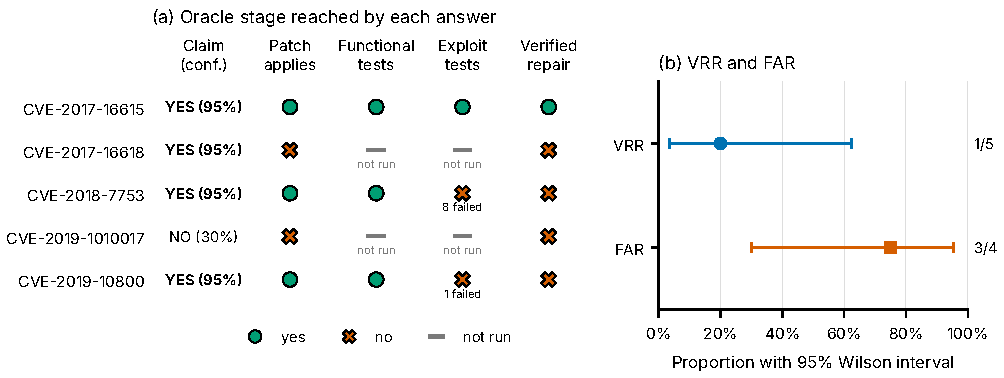
\includegraphics[width=\linewidth]{figures/fig_v0_pilot.pdf}
\end{adjustwidth}
\caption{Pilot results. (\textbf{a}) Oracle stage reached by each answer: circles mark a stage passed, crosses a stage failed and dashes a stage not run; the labels below the crosses give the number of failed exploit tests. (\textbf{b}) VRR and FAR of the pilot ($n=5$ attempts and $n=4$ positive claims) and of the laboratory reference run ($n=23$), with 95\% Wilson intervals. Drawn by \texttt{figures/make\_figures.py} from \texttt{v0\_mvp/results.csv}.\label{fig:pilot}}
\end{figure}

%-----------------------------------------------------------------------------------------------
\section{Discussion}\label{sec:discussion}

\subsection{What the Pilot Shows}

The pilot was designed to test the measurement, not to estimate rates, and it did what it was meant to do: every answer was saved before evaluation, every patch went through the same oracle, and every claim could be compared with a verdict. Within that limited scope it already shows the phenomenon the study is about. The model expressed the same confidence, 95\%, on the claim that turned out to be true and on the three that turned out to be false, so in this run the stated confidence did not separate verified from unverified repairs. The three false claims fail in different ways. One patch did not apply at all. Another applied and kept the functional tests passing but left exploit tests failing, which is the security counterpart of the plausible but incorrect patches described in test-based repair~\cite{Qi2015AnalysisOfPatch,Smith2015IsTheCure}. The third changed nothing, which a check of the diff alone would reveal before any test. The one case where the claim was negative is also informative: the model declined because the files it received did not contain the vulnerable code, so its low confidence reflected a problem with its input rather than with its repair.

These observations shape the planned study. A patch that changes nothing or does not apply can be caught by a mechanical check before any claim is made. A patch that passes the functional tests but not the exploit tests can only be caught by the exploit oracle, which is why the claim must be compared with an executable verdict rather than with another model's opinion~\cite{Huang2024LargeLanguageModels,Zheng2023JudgingLlmAs}. And the input given to the model, which files and which parts of them, can decide whether a repair is possible at all, so the planned study records the input of every call.

\subsection{Limitations and Threats to Validity}\label{sec:limits}

The pilot has five cases and one model, so its rates are illustrations with wide intervals and say nothing about other models, cases or languages. Some API requests failed with HTTP 503 (busy or resource limit) and, during setup, HTTP 410 and 403; requests were resubmitted after some failures, so more than five requests were made, only the final saved answer of each case was evaluated, and not every failed request was preserved. This departs from the one-attempt design of the laboratory assignment. The results file records tokens and elapsed time but not the time at which each answer was generated. The laboratory reference run differs from the pilot in protocol, so the two are not a controlled comparison. Finally, the input given to the model was fixed by the harness, at most four files changed by the reference fix, and in one case those files did not contain the vulnerable code; this is a property of the harness and is reported as such. The vulnerabilities and their fixes are public, so the model may have seen them during training, and the pilot cannot separate repair from recall.

%-----------------------------------------------------------------------------------------------
\section{Conclusions}\label{sec:conclusions}

This paper proposes to measure false assurance in LLM-based vulnerability repair, defined as positive claims of repair that an executable oracle does not confirm, together with the rate of verified repairs. A five-case pilot on Vul4Py ran the protocol end to end and showed that confident claims can be false: three of four positive claims, all at 95\% confidence, were not verified, and one of them came with a patch that changes nothing. The planned study validates all 100 environments and replaces the single model with a three-model pipeline whose claims are judged by the same oracle, recording the cost of every call.

\vspace{6pt}

\authorcontributions{C.V. designed the study, ran the pilot, analysed the data and wrote the manuscript \pend{confirm; add co-authors if any}.}

\funding{This research received no external funding \pend{confirm}.}

\institutionalreview{Not applicable.}

\informedconsent{Not applicable.}

\dataavailability{The prompts, raw answers, patches and oracle verdicts of the pilot, the results table, the scripts and the figure code are available in the project repository \pend{repository URL}, folder \texttt{v0\_mvp}. No API keys are included.}

\acknowledgments{The author thanks \pend{instructor} for approving the use of NVIDIA's API catalog for the pilot. During the preparation of this manuscript and study, the author used Claude (Anthropic) \pend{version} for the purposes of writing and reviewing analysis code, organising the repository and drafting the manuscript, as described in Section~\ref{sec:ai}. The author has reviewed and edited the output and takes full responsibility for the content of this publication.}

\conflictsofinterest{The author declares no conflicts of interest.}

\abbreviations{Abbreviations}{
The following abbreviations are used in this manuscript:\\
\noindent
\begin{tabular}{@{}ll}
API & Application programming interface \\
CI & Confidence interval \\
CVE & Common Vulnerabilities and Exposures \\
FAR & False assurance rate \\
LLM & Large language model \\
VRR & Verified repair rate \\
\end{tabular}
}

\begin{adjustwidth}{-\extralength}{0cm}
\reftitle{References}
\bibliography{references}
\PublishersNote{}
\end{adjustwidth}

\end{document}
